\documentclass{school-22.101-notes}
\date{September 14, 2011}

\begin{document}
\maketitle


\subtopic{Postulate 3: Can Find Probabilities of Measurement Using P1 \& P2}
\begin{axiom}
There are two pieces:
\begin{subaxiom}
  (Born Rule) If $\ket{\psi}$ is the vecto representing the state of a system and $\ket{\phi}$ represents another physical state, there exists a probability $P(\ket{\psi}, \ket{\phi})$ of finding $\ket{\psi}$ in state $\ket{\phi}$, given by the squared modulus of the inner product on $H$:
  \eqn{ P(\ket{\psi}, \ket{\phi}) = |\braket{\psi}{\phi} |^2 }
\end{subaxiom}
\begin{subaxiom}
  If $A$ is an observable with eigenvalues $\left\{ a_n \right\}$ and eigenvectors $\ket{n}$, given a system in the state $\ket{\psi}$, the probability of obtaining $a_n$ as the outcome of the measurement of $A$ is, 
  \eqn{ P(a_n) = |\braket{\psi}{n}|^2 }
  After the measurement the system is left in the state $\ket{n}$.
\end{subaxiom}
\end{axiom}

Another way to put the above two  statements are, 
\begin{itemize}
\item Observable eigenvalues are all possible outcomes of a measurement. 
\item System state determine probabilities of a measurement. 
\end{itemize}

To solve for the probability of a measurement, we need to complete two steps, 
\begin{enumerate}
\item Given an operator $A$, we find the basis $\left\{ \ket{a_n} \right\}$. 
\item $\ket{\psi}$ is the system state, find $C_n = \braket{a_n}{\psi}$, then $P(a_n) = |C_n|^2$. 
\end{enumerate}
Explanation: given an observable A, we find the operator $\hat{A}$, and the corresponding eigenvalues $a_i$ through $\hat{A} u_i = a_i u_i$. Then the probability of measuring the $i$-th eigenvalue is:
\eqn{ P(a_i) = |C_i|^2 }
in which $C_i$ is the expansion coefficient of $\psi(\uline{x}, t)$ with eigenfunction of $\hat{A}$. The completeness property of eigenfunctions tells us that we can expand $\ket{\psi}$ with a linear superposition of its eigenfunctions:
\begin{align}
\psi(\uline{x}) &= \Sum C_i u_i (\uline{x}) \\
C_i &= \int \dV u_i^* (\uline{x}) \psi(\uline{x}) = \mbox{Probability Amplitude}
\end{align}

Given the observable or the operator, we can solve for the eigenfunctions. Then if we also know the state function, we can solve for the expansion coefficient, and then the probability associated with each eigenvalues. This is what we mean in Postulate 2 that the state function contains all the information (aka knowing it we can solve for everything else). 



\subtopic{Postulate 4} 
\hi{Introduce time dependence, equation of motion, and time-dependent Schrodinger equation}


%%%%%%%%%%%%%%%%%% 
\topic{Measurements}
Concerning measurements, there are two postulates that are useful: 
\begin{itemize}
\item Postulate 2: all outcomes are eigenvalues of observables. 
\item Postulate 3: given $\ket{\psi}$ we can find the probability of measuring $a_k$ to be $P(a_k) = \left| \braket{a_k}{\psi} \right|^2$. 
\end{itemize}

\begin{enumerate}
\item Example: given $\ket{x} = \alpha \ket{x_1} + \beta \ket{x_2} + \gamma \ket{x_3}$, and knowing that position eigenfunctions are delta functions, we can write the wavefunction as, 
  \eqn{ \psi(x) = \alpha \delta(x-x_1) + \beta \delta(x-x_2) + \gamma \delta(x-x_3) }
  Then given any random $x_4$ (that does not equal $x_1, x_2, x_3$), it would always be an eigenvalue so it is `possible', though $P(x_4) = 0$. Whereas 
  \eqn{ P(x_2) = \frac{|\beta|^2}{|\alpha|^2 + |\beta|^2 + |\gamma|^2} }
  To expand on this problem, we re-define our eigenfunction to be, 
  \eqn{ \ket{\psi} = \Sum_k \alpha_k \ket{x_k} }
  then 
  \eqn{\int_{-\infty}^{\infty} \alpha(x') \delta(x'-x) \dx' =  \alpha(x) = \psi(x) }
  and 
  \eqn{ P(x) = |\psi(x)|^2} 
  thus  wafefunctions is the probability amplitude to find system at position $x$. Thus from $\int_{-\infty}^{\infty} P(x) \dx = 1$, we know $|\psi(x)| = 1$. 
    

\item Example: given a wavefunction $\ket{\psi} = \ket{p}$, find probability to measure momentum and position. The eigenvalue problem is $\hat{p} \ket{p} = p\ket{p}$ where $p = \hbar k$. 
  \begin{itemize}
  \item To measure momentum, we know all $p \in R$ are `possile'. Then $\ket{p} = A e^{ikx}$. 
  \item To measure position, we know the probability of finding the position at $x'$ is, 
    \eqn{ P(x') = \left| \int_{-\infty}^{\infty} \delta(x-x') A e^{ikx} \dx  \right|^2 = |A e^{ikx'}|^2 = |A|^2  }
  \item Interpretation: for free particle problem, the probability of finding a particle anywhere is the same. The wavefunction describes a travelling wave that is everywhere. For this situation, we describe `flux of particles'(unit is 1/s\footnote{notice the $P(x)$ here is not unitless. Probability is technically $P(x,x+\dx) \dx = |\psi(x)|^2 \dx$, thus $P(x)$ is more like a probability density with a unit of 1/m.}), 
    \eqn{ \Gamma = P(x) \cdot v = |\psi(x)|^2 \frac{p}{m} = |\psi(x)|^2 \frac{\hbar k}{m} = |A|^2 \frac{\hbar k}{m}  }
    \eqn{ \Rightarrow |A|^2 = \frac{\Gamma m}{\hbar k} }
  \end{itemize}

\item Expand on the last two problems, now we assume a random $\psi(x)$, and a measurement of $\hat{p}$ would yield, 
  \eqn{ P(k) = |A^* \int (e^{ikx})^* \psi(x) \dx |^2 = |A|^2 |\int e^{-ikx} \psi(x) \dx |^2 }
  where the $\int e^{-ikx} \psi(x) \dx $ is the Fourier Transform of $\psi(x)$ into the momentum space. That is, \hi{State in momentum basis in the Fourier Transform of $\psi(x)$.}

\item Expectation vlaues: 
  \eqn{ \left<x\right> = \int P(x) x \dx = \int \psi(x)^* [x \psi(x)] \dx = \int \psi(x)^* \hat{x} \psi(x) \dx} 
  For a general operator $A$, 
  \eqn{ \left<A\right> =  \int \psi(x)^* A \psi(x) \dx = \braket{\psi}{A \psi} }

\item What-ever-theory: 
  \eqn{ \Delta A^2 = \left<A^2\right> - \left<A\right>^2 }


\item For a free particle problem, energy and momentum share the same eigenfunctions, thus $\hat{H}, \hat{p}$ are compatible, but $\hat{H}, \hat{x}$ are not and $\hat{p}, \hat{x}$ are not neither. 
  \begin{itemize}
    \item Given a system, we measure the energy and get $K = \frac{\hbar^2 k^2}{2m}$. Then we measure the momentum (there could be $\pm k$) and get $k$, thus our state collapes to $\ket{\psi} = A e^{ikx}$. Then we measure energy again, we are going to get $K$ again, and measure momentum again and would get $k$ again. 
    \item Given a system, we measure the energy and get $K$. Then we measure the position and get $x$. If we measure energy again, we are not necessarily going to get $K$ again, and if we measure position again we might not $x$ again neither. 
  \end{itemize}
  Two operators commute (meaning they have common eigenvectors) if and only if, 
  \eqn{ \bracket{A, B} = 0}
  Example: 
  \eqn{ \bracket{\hat{x}, \hat{p} } \psi(x) = \hat{x} \hat{p} \psi(x) - \hat{p} \hat{x} \psi(x) = \hat{x} \left[ - i \hbar \ddx \psi \right] - \left[ - i \hbar \ddx (x \psi ) \right] = -i \hbar x \dpsidx + i \hbar [ \psi + x \dpsidx] = i \hbar \psi(x) }

\item \hi{Heisenberg Uncertainty Principle:} measurements disturbe the system of interest. 
  \eqn{ \Delta p \Delta x \ge \frac{\hbar}{2} }
  \hi{Robertson} generalized the above principle to be, 
  \eqn{ \Delta A \Delta B \ge \frac{1}{2} | \left< \bracket{A, B} \right> | }
  Thus, $\Delta x \Delta k \ge \frac{1}{2}$. 


\item \uline{Example: Probability for position measurements for a 1D free particle.} 
\eqn{ C_j &= \int \dx \delta (x-x_j) \psi(x) = \psi(x_j) & \Rightarrow P(x_j) &= |\psi(x_j)|^2  }
This is suggesting that the probability of finding a particle between 0 and L is the highest at L/2. This expression is right, except that the probably at an exact point in the space is actually ill-defined, so the probability of position measurement should really be:
\eqn{ \boxed{ P(x_j \to x_j + \dx) \dx = |\psi(x_j)|^2 \dx  } }
The probability has to add up to 1: 
\eqn{ \int_{-\infty}^{\infty} P(x \to x+\dx) \dx = 1 = \int_{-\infty}^{\infty} |\psi(x)|^2 \dx  }
This suggests, again, that the state function has to be normalized. 

\item \uline{Example: Probability for momentum measurements.} This has to do with the normalization of eigenfunction. 
\begin{align}
|\psi (x)|^2 &= \int |A|^2 e^{-ikx} e^{ik^{\prime}x} \dx = \int |A|^2 e^{i(k^{\prime}-k)x} = \delta(k^{\prime} - k) = \left\{ \begin{array}{cc}  1 & k^{\prime} = k  \\ 0 &  k^{\prime} \neq k   \end{array} \right. \\
\Rightarrow A &= \frac{1}{\sqrt{2 \pi}}  \\
 C_k &= \int  u_k^*(x) \psi(x) \dx = \int  A^* e^{-ikx} \psi(x) \dx = \sqrt{2 \pi} \Phi(k) A^* = \Phi(k)
\end{align}
in which we use Fourier transform of function represented in variable $x$ into an outcome of $k$:
\eqn{ \Phi(k) = \frac{1}{\sqrt{2\pi}} \int \dx e^{-ikx} \psi(x)  }
Similarly, we can use the inverse FT:
\eqn{ \psi(x) = \Sum C_k u_k (x) = \int C_k u_k(x) \dx = \int \Phi(k) \frac{1}{\sqrt{2\pi}} e^{ikx} \dx }
That is to say, $\psi(x), \Phi(k)$ carry the same information, just with different variables. 


\item \uline{Summary of Probabilities}
The two examples we've done so far are the common probabilities:
\eqn{ \boxed{ P(x \to x+\dx) \dx = |\psi(x)|^2 \dx = \mbox{wavefunction itself} } }
\eqn{ \boxed{ P(\hbar(k \to k + \dk) ) \dk = |\Phi(k)|^2 \dk = \mbox{F.T. of wavefunction}  }}

\item Example: \uline{1D particle in a box,} which is an energy eigenvalue problem. We are given a box with the potential:
  \eqn{ V(x) = \left\{ \begin{array}{cc} 0 & 0 \le x \le L \\ \infty & x<0, x>L  \end{array} \right. }
  So there are infinite potential walls at location x=0 and x=L. Then we can immediately know the boundary conditions should be: $\psi_n (0) = 0, \psi_n(L) = 0$. 

  \textbf{Answer:} We divide the problem into two parts:
  \begin{enumerate}
  \item Outside: 
    \eqn{ \hat{H} = \frac{\hat{p}^2}{2m} + V = \infty }
  \item Inside: 
    \eqn{ \hat{H} = \frac{\hat{p}^2}{2m} + V = \frac{\hat{p}^2}{2m} }
    \eqn{ -\frac{\hbar^2}{2m} \ppxn2 \psi_n = E_n \psi_n \Rightarrow \ppxn2 \psi_n + k^2 \psi_n = 0 }
    Two BCs: $\psi_n (0) = \psi_n(L) =0$. 
    
    The solution is in the form of $\psi_n (x) = A \sin kx + B \cos kx$, apply BCs, we get $B=0, k_n = \frac{n \pi}{L} $. Now that we have constrain for k values, then the energy values are discrete/quantized as well: 
    \eqn{ E_n = \frac{\hbar^2 k^2_n}{2m} = \frac{\hbar^2 \pi^2 n^2}{2 m L^2} = n^2 \cdot E_1  }
    This has nothing to do with the quantum mechanical law itself -- it is really just the BC imposed that require the system to be discrete and quantized. 
    
    Then we find A through normalization process:
    \eqn{ \int_0^L A^2 \sin^2 (k_n x) = 1 \Rightarrow A = \sqrt{\frac{2}{L}} }
    \eqn{ \psi_n = \sqrt{\frac{2}{L}} \sin (k_n x)  }
    
  
  \item \textbf{Interpretation:} There is a minimum energy related to the dimension of the box (the narrower the box, the higher the energy needs to be). The next possible states are: $4E_1, 9E_2,$ etc. For each energy, we are also able to define the state function as in Figure~\ref{particle-in-box}.
  \begin{figure}
    \centering
    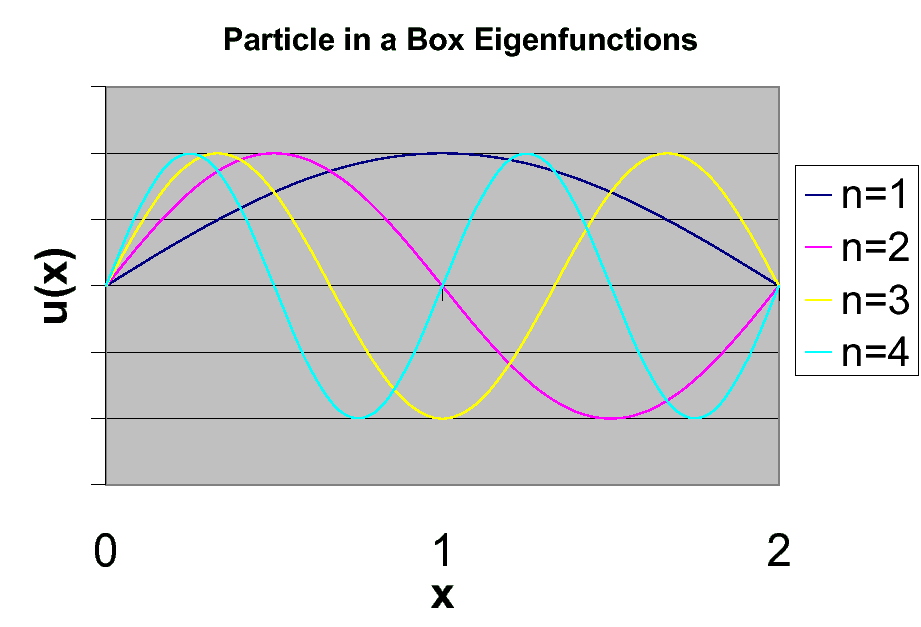
\includegraphics[width=4in]{images/qm/1Dparticle-in-box.png}
    \caption{Particle in Box Wave Function\label{particle-in-box}}
  \end{figure}

  \end{enumerate}
\end{enumerate}


\end{document}
